\documentclass[10pt,twocolumn]{article}

\usepackage[a4paper, margin=2.5cm]{geometry}
\usepackage{amsmath,amssymb}
\usepackage{graphicx}
\usepackage{booktabs}
\usepackage[numbers]{natbib}
\usepackage{hyperref}
\usepackage{algorithm}
\usepackage{algorithmic}
\usepackage{xcolor}
\usepackage{microtype}
\usepackage{bm}
\usepackage{float}

\hypersetup{
  colorlinks=true,
  linkcolor=blue!60!black,
  citecolor=green!50!black,
  urlcolor=blue!70!black
}

\title{Transformer-Brained Artificial Life with Genome-Modulated Attention and Vesicle Communication}

\author{
  Yoichi Ochiai \\
  University of Tsukuba / Digital Nature Group \\
  \texttt{ochiai@digitalnature.slis.tsukuba.ac.jp}
}

\date{}

\begin{document}
\maketitle

% ============================================================================
\begin{abstract}
We present a novel artificial life system in which autonomous agents (``cells'') are governed by a shared Transformer neural controller whose attention mechanism is modulated per-individual by an evolvable genome.
Cells inhabit a toroidal two-dimensional world, forage at spatially distributed nutrient sources, reproduce both asexually and sexually, and communicate by emitting and absorbing \emph{vesicles}---freely diffusing packets of neural state that serve as an indirect, stigmergic channel.
Each cell constructs a token sequence from its own state, the states of its $k$ nearest neighbors augmented with relational features, and nearby vesicle contents, then applies genome-scaled query--key attention to produce movement, emission, and state-update actions.
A comprehensive ablation study across eight conditions (30{,}000 steps, three seeds each) reveals that vesicle communication dramatically reshapes population dynamics: populations with vesicles stabilize at approximately 51 cells versus 280 without, yet exhibit qualitatively richer energy cycling and sustained generational turnover.
Aging pressure is essential for evolutionary progress, while sexual recombination homogenizes genomes.
The genome-modulated attention mechanism significantly alters phenotypic variance, confirming that even without gradient-based learning, evolved attention biases meaningfully differentiate cell behavior.
\end{abstract}

% ============================================================================
\section{Introduction}
\label{sec:intro}

The aspiration of artificial life research is to create systems that exhibit lifelike properties---self-replication, adaptation, ecological dynamics, and open-ended evolution---from minimal mechanistic primitives \cite{langton1990computation,packard2019overview,taylor2016open,bedau2003artificial}.
While classical cellular automata and particle-based models---from von~Neumann's self-reproducing automata \cite{vonneumann1966theory} and Langton's self-replicating loops \cite{langton1984self} to Ray's Tierra system \cite{ray1991approach}---have yielded rich phenomenology, they typically rely on hand-designed update rules that limit the behavioral complexity of individual agents.
Conversely, recent advances in deep reinforcement learning \cite{lowe2017multi} have produced sophisticated individual agents, yet these systems rarely exhibit the emergent ecological and evolutionary dynamics that characterize biological communities.

In this work, we bridge these two traditions by constructing an artificial life system whose agents are controlled by a Transformer architecture \cite{vaswani2017attention}---the same class of model that has driven recent advances in language understanding, vision, and decision-making.
Our key insight is that the multi-head self-attention mechanism provides a natural substrate for relational reasoning about neighboring agents and environmental signals, and that the attention parameters themselves can be made a target of evolution.

We introduce three principal contributions:

\begin{enumerate}
\item \textbf{Genome-modulated attention.} Each cell carries an evolvable genome vector that modulates the per-head query and key scaling factors of the shared Transformer brain, producing heritable phenotypic variation without requiring separate weight evolution.

\item \textbf{Vesicle-mediated stigmergic communication.} Cells emit freely diffusing vesicles that carry neural state vectors through the environment. Nearby vesicles enter the attention context as additional tokens, enabling indirect communication that is spatially and temporally decoupled from the emitter.

\item \textbf{Integrated evolutionary ecology.} Asexual division, sexual recombination with genome-similarity gating, predation, speciation pressure, aging, and nutrient competition are unified in a single energy-based economy, enabling systematic ablation of each mechanism.
\end{enumerate}

We evaluate the system through a comprehensive ablation study involving eight experimental conditions, each run for 30{,}000 steps across three random seeds. Our results demonstrate that vesicle communication, while reducing steady-state population size, fundamentally reshapes the evolutionary and energetic dynamics of the population. We find that aging pressure is indispensable for generational turnover, that sexual recombination reduces rather than increases genome diversity, and that genome-modulated attention produces measurable effects on phenotypic variance.

The remainder of this paper is organized as follows. Section~\ref{sec:related} surveys related work in neural artificial life, emergent communication, and neuroevolution. Section~\ref{sec:model} formalizes the model architecture and dynamics. Section~\ref{sec:experiments} describes the experimental setup. Section~\ref{sec:results} presents and analyzes the ablation results. Section~\ref{sec:discussion} discusses implications and limitations, and Section~\ref{sec:conclusion} concludes.


% ============================================================================
\section{Related Work}
\label{sec:related}

\paragraph{Neural cellular automata.}
Mordvintsev et al.\ \cite{mordvintsev2020growing} introduced Growing Neural Cellular Automata (NCA), demonstrating that a small convolutional network applied uniformly at each grid cell can learn to grow and regenerate complex patterns through gradient-based training.
Zhang et al.\ \cite{zhang2025petridish} extended this paradigm with Petri Dish NCA, evolving NCA rules to produce virtual creatures with diverse morphologies.
Indirect encoding approaches such as HyperNEAT \cite{stanley2009hypercube} have been used to evolve large-scale neural network connectivity patterns, while Gaier and Ha \cite{gaier2019weight} demonstrated that network topology alone---without weight training---can produce capable agents, highlighting the importance of architecture over parameters.
Our work differs fundamentally in that agents are mobile particles rather than grid-fixed cells, and the neural controller uses attention over a variable-length neighbor set rather than convolution over a fixed local neighborhood.

\paragraph{Particle-based artificial life.}
The ALIEN simulator \cite{alien2024} is a GPU-accelerated artificial life platform supporting soft-body physics, neural network controllers, and self-replicating organisms, achieving populations of millions of cells.
Lenia \cite{chan2019lenia} and its extension Flow-Lenia \cite{plantec2025flow} define continuous cellular automata with smooth, kernel-based update rules that produce strikingly lifelike patterns.
While Lenia operates on continuous fields, our system models discrete agents with individual neural controllers, genomes, and energy budgets.
Neural MMO \cite{suarez2023neural} provides a massively multiagent game environment, but agents therein are trained via reinforcement learning rather than evolved.

\paragraph{Emergent communication.}
The study of emergent communication in multi-agent systems has a rich history.
Lazaridou et al.\ \cite{lazaridou2017multi} showed that agents trained with reinforcement learning can develop referential communication protocols, though Kottur et al.\ \cite{kottur2017natural} cautioned that natural language does not emerge naturally without appropriate inductive biases.
Foerster et al.\ \cite{foerster2016learning} demonstrated that agents can learn to communicate through differentiable channels; Mordatch and Abbeel \cite{mordatch2018emergence} showed grounded compositional language can emerge in multi-agent populations, and Eccles et al.\ \cite{eccles2019biases} identified key biases that facilitate emergent communication.
Stigmergic communication---indirect coordination through environmental modification---has been explored in multi-agent reinforcement learning by Wang et al.\ \cite{wang2019sigrl} and Zheng et al.\ \cite{zheng2022pool}, drawing on biological inspiration from pheromone-based insect coordination \cite{bonabeau1999swarm} and the self-organization principles observed in flocking \cite{reynolds1987flocks} and swarm systems \cite{camazine2001self}.
Our vesicle mechanism is most closely related to stigmergic approaches, but the vesicles carry high-dimensional neural state vectors rather than scalar signals, enabling richer information transfer.

\paragraph{Neuroevolution and evolved attention.}
The evolution of neural network topologies and weights has a long history beginning with NEAT \cite{stanley2002evolving} and its indirect encoding extension HyperNEAT \cite{stanley2009hypercube}.
Sims \cite{sims1994evolving} pioneered the co-evolution of morphology and neural control.
Tang et al.\ \cite{tang2020neuroevolution} evolved attentional mechanisms for self-interpretable agents, demonstrating that attention weights can serve as a readable trace of agent decision-making.
Ha \cite{ha2019reinforcement} explored the design of agent bodies through reinforcement learning.
Salimans et al.\ \cite{salimans2017evolution} showed that evolution strategies scale competitively with reinforcement learning, while Such et al.\ \cite{such2017deep} demonstrated that deep neuroevolution via genetic algorithms can match gradient-based methods without backpropagation.
Gaier and Ha \cite{gaier2019weight} further showed that weight-agnostic neural networks---where topology matters more than weight values---can solve reinforcement learning tasks, providing a conceptual contrast to our genome-modulated approach where shared weights are reinterpreted through per-agent scaling.
Our genome-modulated attention differs from prior neuroevolution approaches in that the network weights are shared across all agents; evolution acts only on a compact genome vector that multiplicatively scales the query and key projections, providing a biologically inspired analog of epigenetic regulation.

\textbf{ALife as visual medium.}
The tradition of ALife visualization as both scientific tool and aesthetic object dates to Sims' \emph{Evolved Virtual Creatures}~\cite{sims1994evolving}, where the visual richness of evolved morphologies was itself a primary contribution.
More recently, systems like Lenia~\cite{chan2019lenia} and ALIEN~\cite{alien2024} have demonstrated that real-time visualization can reveal emergent phenomena invisible in quantitative analysis alone.
McCormack and d'Inverno~\cite{mccormack2012computers} argued that computational creativity and artificial life share deep structural concerns: both study systems that generate novelty from simple rules.
Our visualization design follows this tradition, treating the renderer not as a post-hoc display but as an integral part of the system's epistemic and aesthetic contribution.


% ============================================================================
\section{Model}
\label{sec:model}

We describe the complete model in six subsections: the world representation (Section~\ref{sec:world}), the Transformer brain architecture (Section~\ref{sec:brain}), vesicle communication (Section~\ref{sec:vesicle}), the energy economy (Section~\ref{sec:energy}), evolutionary operators (Section~\ref{sec:evolution}), and real-time visualization (Section~\ref{sec:visualization}).

% --------------------------------------------------------------------------
\subsection{World and Cell Representation}
\label{sec:world}

The world $\mathcal{W}$ is a toroidal two-dimensional domain of size $W_x \times W_y$ (default $1080 \times 800$ pixels), following the tradition of spatial agent models where boundary-free topology avoids edge artifacts \cite{reynolds1987flocks,vicsek1995novel}.
All distance computations use the wrapped (toroidal) metric:
\begin{equation}
  d_w(\mathbf{p}_i, \mathbf{p}_j) = \left\| \min\!\big(|\mathbf{p}_i - \mathbf{p}_j|,\; \mathbf{W} - |\mathbf{p}_i - \mathbf{p}_j|\big) \right\|_2
\end{equation}
where $\mathbf{W} = [W_x, W_y]^T$ and operations are element-wise.

Each cell $i$ in the population $\mathcal{C}$ (with $|\mathcal{C}| \leq C_{\max} = 700$) is characterized by:
\begin{itemize}
  \item \textbf{State} $\mathbf{s}_i \in \mathbb{R}^{D}$ ($D = 32$): the cell's internal neural state, serving as both its ``phenotype'' and its working memory.
  \item \textbf{Genome} $\mathbf{g}_i \in \mathbb{R}^{G}$ ($G = 16$): a heritable vector that modulates the attention mechanism and participates in inter-cell interactions.
  \item \textbf{Position} $\mathbf{p}_i \in \mathbb{R}^{2}$: spatial coordinates in the toroidal world.
  \item \textbf{Velocity} $\mathbf{v}_i \in \mathbb{R}^{2}$: current movement vector, subject to momentum.
  \item \textbf{Energy} $e_i \in \mathbb{R}$: a scalar resource that governs survival, reproduction, and vesicle emission.
  \item \textbf{Age} $a_i \in \mathbb{N}$: the number of simulation steps since the cell's creation.
  \item \textbf{Generation} $\ell_i \in \mathbb{N}$: the cell's lineage depth (incremented at each reproduction event).
\end{itemize}

The world also contains $N_{\text{nut}}$ nutrient sources (default 16), each at a fixed position with a signature vector $\hat{\mathbf{n}}_k \in \mathbb{R}^D$, radius $r_n = 200$, and a depletable energy reserve.


% --------------------------------------------------------------------------
\subsection{Transformer Brain}
\label{sec:brain}

All cells share a single Transformer neural controller (the ``brain'') whose weights are fixed throughout the simulation---there is no gradient-based learning.
Behavioral differentiation arises entirely from differences in state, genome, and local context.
The brain takes as input a variable-length token sequence constructed from the cell's own state, its neighbors' states, and nearby vesicle contents, and produces an action vector.

\subsubsection{Token Sequence Construction}

For cell $i$, the self-token is constructed by projecting the genome into state space and applying layer normalization:
\begin{equation}
  \mathbf{x}_i = \text{LN}\!\big(\mathbf{s}_i + W_g \mathbf{g}_i\big)
  \label{eq:self_token}
\end{equation}
where $W_g \in \mathbb{R}^{D \times G}$ is a learned projection matrix and $\text{LN}(\cdot)$ denotes layer normalization \cite{ba2016layer}.

\subsubsection{Relational Features}

We identify the $k = 6$ nearest neighbors $\mathcal{N}_i = \{j_1, \ldots, j_k\}$ by wrapped Euclidean distance.
For each neighbor $j_l$, we compute a relational feature vector encoding spatial and kinematic relationships:
\begin{equation}
  \mathbf{r}_{i,l} = W_r \begin{bmatrix} \Delta p_x / 100 \\ \Delta p_y / 100 \\ d_{i,l} / 200 \\ \Delta v_x / 5 \\ \Delta v_y / 5 \end{bmatrix}
  \label{eq:rel_features}
\end{equation}
where $\Delta p_x, \Delta p_y$ are the wrapped relative position components, $d_{i,l} = d_w(\mathbf{p}_i, \mathbf{p}_{j_l})$ is the wrapped distance, $\Delta v_x, \Delta v_y$ are relative velocity components, and $W_r \in \mathbb{R}^{D \times 5}$ is a learned projection.
The normalization constants (100, 200, 5) keep the inputs in a numerically stable range.

Each neighbor token is formed by adding the relational embedding to the neighbor's raw state:
\begin{equation}
  \tilde{\mathbf{s}}_{j_l} = \mathbf{s}_{j_l} + \mathbf{r}_{i,l}
  \label{eq:neighbor_token}
\end{equation}

Up to $m = 3$ vesicle tokens $\mathbf{c}_{v_1}, \ldots, \mathbf{c}_{v_m}$ are included from vesicles within a sensing radius of $2 \times r_a = 52$ pixels (Section~\ref{sec:vesicle}).

The complete token sequence is:
\begin{equation}
  \mathbf{Z} = [\mathbf{x}_i,\; \tilde{\mathbf{s}}_{j_1}, \ldots, \tilde{\mathbf{s}}_{j_k},\; \mathbf{c}_{v_1}, \ldots, \mathbf{c}_{v_m}]
  \label{eq:token_seq}
\end{equation}
with a maximum sequence length of $L = 1 + k + m = 10$. Positions without valid tokens (fewer neighbors or vesicles) are masked.

\subsubsection{Genome-Modulated Attention}

The central architectural novelty is that the cell's genome multiplicatively modulates the query and key projections on a per-head basis.
Given $H = 4$ attention heads with head dimension $d_h = D/H = 8$, we compute genome-dependent scaling factors:
\begin{equation}
  [\bm{\alpha}_q,\; \bm{\alpha}_k] = \sigma\!\big(W_{qk}\, \mathbf{g}_i\big) \in \mathbb{R}^{2H}
  \label{eq:genome_scale}
\end{equation}
where $W_{qk} \in \mathbb{R}^{2H \times G}$ is a learned projection and $\sigma(\cdot)$ is the sigmoid function, ensuring the scaling factors lie in $(0, 1)$.

The query is computed from the self-token only, while keys and values are computed from the full token sequence $\mathbf{Z}$:
\begin{align}
  Q^{(h)} &= \alpha_q^{(h)} \cdot W_Q^{(h)}\, \mathbf{x}_i \label{eq:query} \\
  K^{(h)} &= \alpha_k^{(h)} \cdot W_K^{(h)}\, \mathbf{z}_l \quad \forall\, \mathbf{z}_l \in \mathbf{Z} \label{eq:key} \\
  V^{(h)} &= W_V^{(h)}\, \mathbf{z}_l \quad \forall\, \mathbf{z}_l \in \mathbf{Z} \label{eq:value}
\end{align}
where $W_Q^{(h)}, W_K^{(h)}, W_V^{(h)} \in \mathbb{R}^{d_h \times D}$ are head-specific projection matrices.

The scalar factors $\alpha_q^{(h)}, \alpha_k^{(h)} \in (0,1)$ allow the genome to selectively amplify or suppress individual attention heads, providing a form of evolved attentional bias analogous to epigenetic regulation.
When $\alpha_q^{(h)} \approx 0$, head $h$ is effectively silenced for cell $i$; when $\alpha_q^{(h)} \approx 1$, head $h$ operates at full capacity.

\subsubsection{Attention Computation}

Attention scores are computed with causal masking for padded positions:
\begin{equation}
  A^{(h)} = \text{softmax}\!\left(\frac{Q^{(h)} {K^{(h)}}^T}{\sqrt{d_h}} + M\right)
  \label{eq:attention}
\end{equation}
where $M_l = -\infty$ for padded (masked) positions and $M_l = 0$ otherwise.

The multi-head output is concatenated and linearly projected:
\begin{equation}
  \mathbf{o}_i = W_o [\text{head}^{(1)} \| \cdots \| \text{head}^{(H)}]
  \label{eq:mha_output}
\end{equation}
where $\text{head}^{(h)} = A^{(h)} V^{(h)}$ and
where $W_o \in \mathbb{R}^{D \times D}$ is the output projection.

A residual connection and a feed-forward block with GELU activation and a second layer normalization complete the Transformer layer:
\begin{equation}
  \mathbf{h}_i = \mathbf{x}_i + \mathbf{o}_i, \quad
  \mathbf{a}_i = \text{FFN}\!\big(\text{LN}(\mathbf{h}_i)\big) + \mathbf{h}_i
  \label{eq:ffn}
\end{equation}
where $\text{FFN}(\mathbf{z}) = W_2\, \text{GELU}(W_1 \mathbf{z})$ with $W_1 \in \mathbb{R}^{2D \times D}$ and $W_2 \in \mathbb{R}^{D \times 2D}$.

\subsubsection{Action Decoding}

A final linear head maps $\mathbf{a}_i$ to the action vector $[a_1, \ldots, a_{D+4}] = W_h \mathbf{a}_i$, which is decoded as:
\begin{align}
  \Delta x, \Delta y &= 2.5 \cdot \tanh(a_1, a_2) \label{eq:action_move} \\
  p_{\text{emit}} &= \sigma(a_3) \label{eq:action_emit} \\
  \alpha &= 0.25 \cdot \sigma(a_4) \label{eq:action_alpha} \\
  \mathbf{c}_{\text{emit}} &= [a_5, \ldots, a_{D+4}] \in \mathbb{R}^D \label{eq:action_content}
\end{align}
The four outputs correspond to movement displacement, vesicle emission probability, state blend factor, and vesicle content vector, respectively.

Velocity is updated with momentum: $\mathbf{v}_i^{t+1} = 0.6\, [\Delta x, \Delta y]^T + 0.4\, \mathbf{v}_i^t$, and the position is updated modulo the world dimensions.


% --------------------------------------------------------------------------
\subsection{Vesicle Communication}
\label{sec:vesicle}

Vesicles are freely diffusing packets of neural state that enable indirect (stigmergic) communication between cells.
The vesicle pool supports up to $V_{\max} = 3{,}000$ simultaneous vesicles.

\paragraph{Emission.}
Cell $i$ emits a vesicle with probability $p_{\text{emit}}$ (Eq.~\ref{eq:action_emit}), gated by an energy threshold to prevent emission during starvation ($e_i > e_{\text{starve}} = 40$).
The vesicle is initialized at the cell's position with a random emission direction:
\begin{equation}
  \mathbf{p}_v = \mathbf{p}_i, \quad
  \mathbf{v}_v = v_{\text{spd}} \begin{bmatrix} \cos\theta \\ \sin\theta \end{bmatrix}, \quad
  \mathbf{c}_v = \mathbf{c}_{\text{emit}}
  \label{eq:vesicle_emit}
\end{equation}
where $\theta \sim \text{Uniform}(0, 2\pi)$ and $v_{\text{spd}} = 1.3$. Emission costs the cell $C_{\text{emit}} = 0.06$ energy units.

\paragraph{Dynamics.}
Vesicles undergo Brownian drift with viscous damping:
\begin{align}
  \mathbf{p}_v^{t+1} &= \big(\mathbf{p}_v^{t} + \mathbf{v}_v^{t} + \bm{\epsilon}\big) \bmod \mathbf{W}, \quad \bm{\epsilon} \sim \mathcal{N}(\mathbf{0},\, 0.04\, \mathbf{I}) \label{eq:vesicle_pos} \\
  \mathbf{v}_v^{t+1} &= 0.994 \cdot \mathbf{v}_v^{t} \label{eq:vesicle_vel}
\end{align}
Vesicles have a finite lifetime of $\tau_v = 150$ steps, after which they are removed.

\paragraph{Absorption.}
When a vesicle $v$ comes within an absorption radius $r_a = 26$ pixels of any cell $j$ (using wrapped distance), the nearest cell absorbs it.
Absorption modifies the cell's internal state through a masked, nonlinear blending operation:
\begin{equation}
  \mathbf{s}_j \leftarrow (1 - \beta \cdot \mathbf{m}) \odot \mathbf{s}_j + (\beta \cdot \mathbf{m}) \odot \mathbf{c}_v
  \label{eq:vesicle_absorb}
\end{equation}
where $\mathbf{m} \in \{0, 1\}^D$ is a \emph{write mask} defined by $m_d = \mathbf{1}[|c_{v,d}| > 0.3]$ (only dimensions with sufficiently strong signal are written), and $\beta$ is an adaptive blend factor:
\begin{equation}
  \beta = \begin{cases} 0.5 & \text{if recent absorptions} > 3 \\ 0.3 & \text{otherwise} \end{cases}
  \label{eq:blend_factor}
\end{equation}
The ``recent absorptions'' counter decays exponentially ($\times 0.95$ per step), implementing a form of short-term memory that increases receptivity to vesicle signals during periods of high vesicle flux.

\paragraph{Vesicles as attention tokens.}
Beyond direct state modification through absorption, vesicles also serve as context for the Transformer brain.
The biological inspiration draws from extracellular vesicle research, which has revealed that exosomes, microvesicles, and other secreted particles carry rich molecular cargo between cells, modulating recipient behavior at a distance \cite{raposo2013extracellular,tkach2016communication,vanniel2018shedding}.
Up to three vesicles within the sensing radius ($2 r_a = 52$ pixels) are included as additional tokens in the attention sequence (Eq.~\ref{eq:token_seq}), allowing cells to ``perceive'' nearby vesicles before absorbing them and adjust their behavior accordingly.


% --------------------------------------------------------------------------
\subsection{Energy Economy}
\label{sec:energy}

Energy is the universal currency governing survival, reproduction, and communication. The energy update at each step is:
\begin{multline}
  e_i^{t+1} = e_i^t + \rho_{\text{passive}} - \delta_{\text{decay}} - \mu \|\mathbf{v}_i\| \\
  + G_i^{\text{nut}} - C_i^{\text{emit}} - P_i^{\text{age}} - P_i^{\text{crowd}}
  \label{eq:energy}
\end{multline}
where the terms are defined as follows.

\paragraph{Passive regeneration.}
All cells receive a small background energy gain $\rho_{\text{passive}} = 0.012$ per step, preventing immediate extinction in nutrient-poor regions.

\paragraph{Metabolic decay.}
A constant drain $\delta_{\text{decay}} = 0.003$ represents basal metabolism.

\paragraph{Movement cost.}
Locomotion is penalized proportionally to speed: $\mu\, \|\mathbf{v}_i\|$ with $\mu = 0.005$.

\paragraph{Nutrient gain.}
When cell $i$ is within the radius $r_n$ of nutrient source $k$, it receives:
\begin{multline}
  G_i^{\text{nut}} = \frac{\gamma}{N_{\text{feeders}}} \cdot \big(0.6 + 0.4 \cdot \cos(\hat{\mathbf{s}}_i, \hat{\mathbf{n}}_k)\big) \\
  \cdot \left(1 - \frac{d_{ik}}{r_n}\right)^{\!+}
  \label{eq:nutrient}
\end{multline}
where $\gamma = 0.5$ is the base nutrient gain, $\cos(\hat{\mathbf{s}}_i, \hat{\mathbf{n}}_k)$ is the cosine similarity between the cell's expressed phenotype and the nutrient's signature vector (implementing a form of niche specialization), and $N_{\text{feeders}}$ is the number of cells concurrently feeding at that source (implementing scramble competition). The $(1-d/r_n)^+$ term creates a distance-based falloff. Nutrient sources are also depletable, with energy regenerating at 0.08 per step up to a maximum of 100.

\paragraph{Emission cost.}
$C_i^{\text{emit}} = 0.06$ per vesicle emitted.

\paragraph{Aging pressure.}
Cells incur increasing metabolic costs as they age:
\begin{equation}
  P_i^{\text{age}} = 0.05 \cdot \frac{\max(0,\; a_i - 4000)}{8000}
  \label{eq:aging}
\end{equation}
This ramp imposes no penalty before age 4{,}000, then linearly increases, ensuring that even well-fed cells eventually die and yield population turnover.

\paragraph{Crowding penalty.}
Cells whose nearest neighbor is within 15 pixels pay a small penalty:
\begin{equation}
  P_i^{\text{crowd}} = 0.005 \cdot \mathbf{1}[d_{\text{nn}} < 15]
  \label{eq:crowding}
\end{equation}

Cells die when $e_i \leq 0$. A minimum population floor of 10 cells is maintained by respawning near nutrient sources when the population drops below this threshold.


% --------------------------------------------------------------------------
\subsection{Evolutionary Operators}
\label{sec:evolution}

The system supports four evolutionary mechanisms, each operating through the energy economy.
The design draws on foundational principles of genetic algorithms \cite{holland1992adaptation,goldberg1989genetic}.

\paragraph{Asexual division.}
When a cell's energy exceeds the division threshold $E_{\text{div}} = 88$, it produces a daughter cell:
\begin{align}
  \mathbf{g}_{\text{child}} &= \mathbf{g}_i + \bm{\epsilon}_m, \quad \bm{\epsilon}_m \sim \mathcal{N}(\mathbf{0},\, \sigma_m^2 \mathbf{I}), \quad \sigma_m = 0.04 \label{eq:asexual_genome} \\
  e_i &\leftarrow 0.45 \cdot e_i, \quad e_{\text{child}} = 0.45 \cdot e_i \label{eq:asexual_energy}
\end{align}
The child inherits the parent's state vector and is placed nearby (Gaussian offset with $\sigma = 15$ pixels). The remaining 10\% of the parent's pre-division energy is lost to the ``cost of reproduction.''

\paragraph{Sexual recombination.}
Two cells $i$ and $j$ may reproduce sexually when all of the following conditions are met: (i) both have energy $> 0.7 \cdot E_{\text{div}}$, (ii) $\|\mathbf{p}_i - \mathbf{p}_j\|_w < 20$ pixels, and (iii) their genomes have moderate similarity $0.3 < \cos(\mathbf{g}_i, \mathbf{g}_j) < 0.7$.
The similarity window prevents both self-cloning (too similar) and interspecies hybridization (too different).
Given eligible parents, recombination occurs with probability 0.02 per step:
\begin{equation}
  g_{\text{child},d} = \begin{cases}
    g_{i,d} & \text{w.p.\ } 0.5 \\
    g_{j,d} & \text{w.p.\ } 0.5
  \end{cases} + \epsilon_{m,d}
  \label{eq:sexual_genome}
\end{equation}
Each parent loses 30\% of its energy, and the child receives $0.8 \times E_{\text{init}}$ energy.

\paragraph{Speciation pressure.}
To discourage genomic homogeneity and promote diversification, cells in genetically uniform neighborhoods incur a small energy drain:
\begin{equation}
  e_i \leftarrow e_i - 0.003 \cdot \mathbf{1}\!\big[\bar{\cos}(\mathbf{g}_i, \mathbf{g}_{\mathcal{N}_i}) > 0.8\big]
  \label{eq:speciation}
\end{equation}
where $\bar{\cos}(\mathbf{g}_i, \mathbf{g}_{\mathcal{N}_i})$ is the mean cosine similarity between cell $i$'s genome and the genomes of its $k$ nearest neighbors.

\paragraph{Predation.}
When two cells have strongly dissimilar genomes ($\cos(\mathbf{g}_i, \mathbf{g}_j) < -0.5$), a predation event may occur with probability 0.05 per step:
\begin{equation}
  e_{\text{predator}} \leftarrow e_{\text{predator}} + 0.1, \quad e_{\text{prey}} \leftarrow e_{\text{prey}} - 0.15
  \label{eq:predation}
\end{equation}
The asymmetric transfer (prey loses more than predator gains) models metabolic inefficiency and creates selective pressure for genome divergence.


\subsection{Real-Time Visualization}
\label{sec:visualization}

The renderer maps internal simulation state onto visual channels that make emergent dynamics immediately legible (Figure~\ref{fig:visual}).
Each cell is drawn as a \emph{transparent polygonal membrane} with $n$-vertex organic deformation:
\begin{equation}
  r_j(\theta) = R_{\text{base}} \bigl(1 + \eta(\theta; \mathbf{g}_i, \mathbf{s}_i, a_i)\bigr) \cdot \bigl(1 + \lambda \cos(\theta - \phi_v)\bigr)
\end{equation}
where $R_{\text{base}} \propto e_i$ scales with energy (larger = more energetic), $\eta$ is a low-frequency noise function seeded by genome and state (giving each cell a unique silhouette), and $\lambda \cos(\theta - \phi_v)$ stretches the membrane along the velocity direction $\phi_v$, producing a fluid-dynamic deformation analogous to biological cell motility.

\textbf{Color encoding.}
Cell hue is determined by the first four components of the state vector $\mathbf{s}_i$ via an HSV mapping with full $360^\circ$ hue range and high saturation ($\geq 0.75$), ensuring that phenotypically similar cells are chromatically grouped while distinct phenotypes are visually separable.
Membrane outlines exhibit \emph{iridescence}: RGB components oscillate sinusoidally with simulation time and cell index, mimicking the thin-film interference observed in biological lipid bilayers~\cite{vanniel2018shedding}.

\textbf{Nutrient zones} are rendered as multi-layered translucent cloud sprites with pulsing radial animation, visually encoding the resource landscape.
The nutrient signature determines the cloud's hue, establishing a visual connection between nutrient identity and the phenotypic colors of cells that specialize on them.

\textbf{Vesicle trails} appear as tapered streaks with velocity-dependent length and brightness proportional to remaining lifetime, creating a visible ``chemical field'' that conveys the spatial pattern of inter-cell signaling.

\textbf{DNA barcode panel.}
The right-side panel displays genome ($G = 16$ channels) and expressed phenotype (first 16 state dimensions) as horizontal color-coded barcodes, sorted by nutrient-cluster assignment.
This juxtaposition enables visual detection of speciation events: when a contiguous cluster of barcodes develops a distinct color pattern, a new lineage has emerged.
Cluster boundaries are marked with colored tags matching the nutrient source, linking spatial ecology to genomic structure.

\textbf{Synaptic network.}
Faint lines connect each cell to its three nearest neighbors (distance $< 45$ pixels), rendering the implicit neighbor graph that underlies the Transformer's attention computation.
Line opacity decreases with distance, creating a visual analog of attention strength.

The visualization design follows the principle of \emph{double legibility}~\cite{bedau2003artificial}: the system must be scientifically analyzable \emph{and} visually engaging.
The transparent lens aesthetic---inspired by microscopy of living cells---produces emergent visual complexity (overlapping membranes create Moir\'{e}-like interference patterns) that rewards sustained observation and makes the simulation function as both a scientific instrument and a generative artwork.

\begin{figure}[t]
\centering
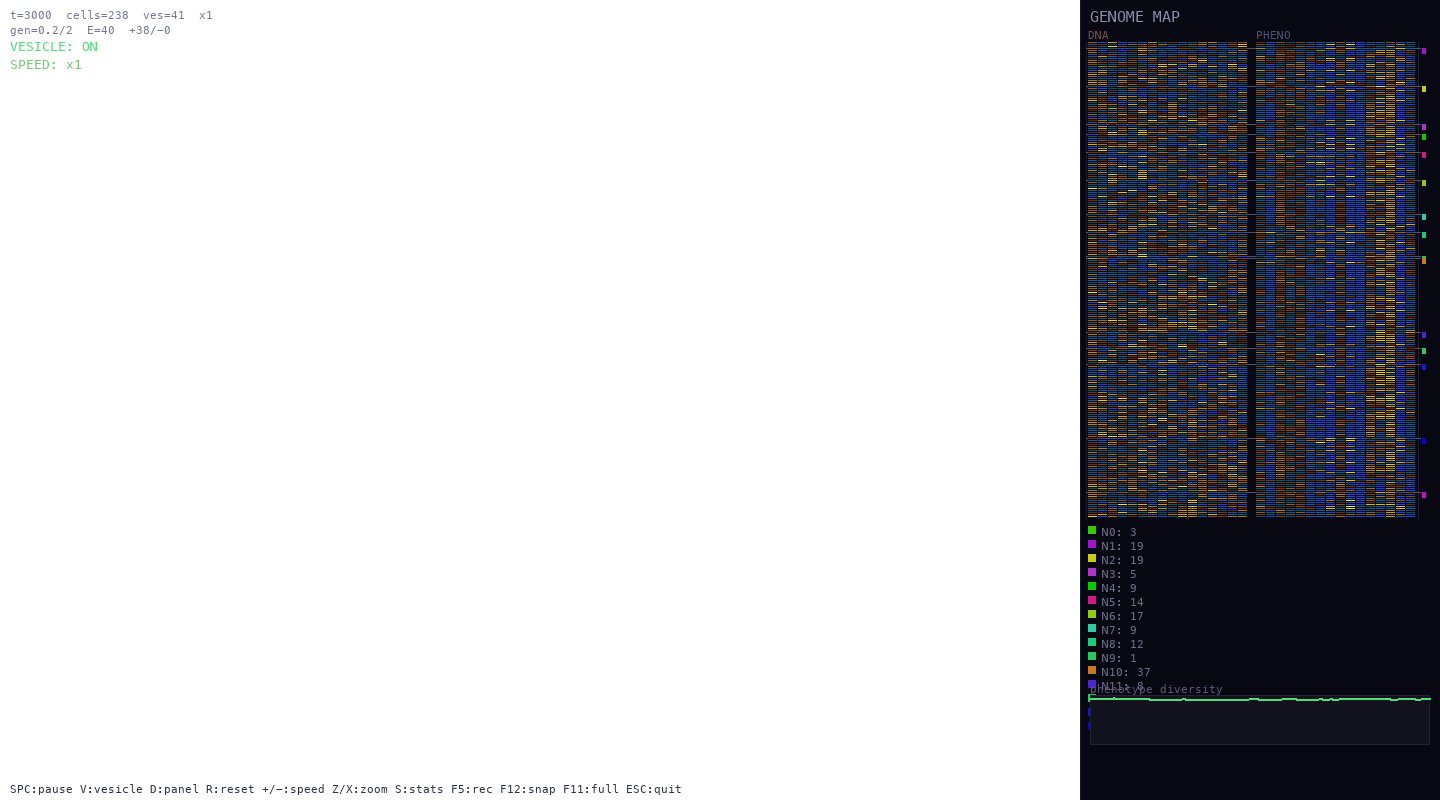
\includegraphics[width=\columnwidth]{docs/screenshot.png}
\caption{Real-time visualization at step 3000. Transparent lens cells cluster around cloudy nutrient zones, with iridescent membranes encoding phenotype. Right: DNA barcode panel showing genome (left column) and expressed phenotype (right column) sorted by nutrient cluster. Faint synaptic lines reveal the neighbor topology.}
\label{fig:visual}
\end{figure}


% ============================================================================
\section{Experimental Setup}
\label{sec:experiments}

\subsection{Ablation Conditions}

To isolate the contribution of each mechanism, we define eight experimental conditions:

\begin{enumerate}
  \item \textbf{Full System}: All mechanisms active (vesicles, genome modulation, sexual recombination, predation, speciation pressure, aging).
  \item \textbf{No Vesicle}: Vesicle communication disabled (no emission, absorption, or vesicle tokens in attention).
  \item \textbf{No Genome Mod}: Genome modulation of attention disabled; query/key scaling factors fixed at 0.5 for all heads and all cells.
  \item \textbf{No Sexual}: Sexual recombination disabled; only asexual division is available.
  \item \textbf{No Predation}: Predation interactions disabled.
  \item \textbf{No Speciation}: Speciation pressure (genome similarity drain) disabled.
  \item \textbf{No Aging}: Aging pressure disabled; cells can live indefinitely if energy permits.
  \item \textbf{Minimal}: No vesicle, no sexual recombination, and no predation; a minimal baseline with only asexual division, speciation pressure, and aging.
\end{enumerate}

\subsection{Protocol}

Each condition is run for 30{,}000 simulation steps with three random seeds ($s \in \{0, 1, 2\}$), yielding 24 independent runs.
The world is initialized with $N_{\text{init}} = 200$ cells scattered near 16 randomly placed nutrient sources, with initial energy $e_0 = 80$.
All conditions use identical random initial weights for the Transformer brain.
Wall-clock time averages approximately 290 seconds per run on a single CPU core.

\subsection{Metrics}

We track the following quantities at each step and report summary statistics (mean $\pm$ standard deviation) computed over the final 10\% of each run (steps 27{,}000--30{,}000):

\begin{itemize}
  \item \textbf{Population size}: number of alive cells.
  \item \textbf{Genome variance}: $\text{Var}(\mathbf{g})$, the sum of per-dimension variances of genome vectors across all alive cells.
  \item \textbf{Phenotype variance}: $\text{Var}(\mathbf{s})$, the analogous quantity for state vectors.
  \item \textbf{Active vesicles}: number of alive vesicles (for conditions with vesicles).
  \item \textbf{Maximum generation}: highest lineage depth among alive cells.
  \item \textbf{Total births and deaths}: cumulative counts over the full run.
\end{itemize}

\subsection{Parameters}

Table~\ref{tab:params} summarizes all simulation parameters.

\begin{table}[t]
\centering
\small
\caption{Simulation parameters.}
\label{tab:params}
\begin{tabular}{@{}llr@{}}
\toprule
\textbf{Cat.} & \textbf{Parameter} & \textbf{Val.} \\
\midrule
World & Size $W_x \!\times\! W_y$ & $1080\!\times\!800$ \\
      & Max cells $C_{\max}$ & 700 \\
      & Max vesicles $V_{\max}$ & 3000 \\
      & Initial cells $N_{\text{init}}$ & 200 \\
\midrule
Neural & State dim $D$ & 32 \\
       & Genome dim $G$ & 16 \\
       & Heads $H$ / Neighbors $k$ & 4 / 6 \\
       & Vesicle tokens $m$ & 3 \\
\midrule
Energy & Init.\ energy $e_0$ & 80 \\
       & Division $E_{\text{div}}$ & 88 \\
       & Passive regen & 0.012 \\
       & Decay / Move cost & 0.003 / 0.005 \\
       & Nutrient gain $\gamma$ & 0.5 \\
       & Nutrient radius $r_n$ & 200 \\
\midrule
Vesicle & Speed / Lifetime & 1.3 / 150 \\
        & Emit cost / Abs.\ radius & 0.06 / 26 \\
        & Damping / Brownian $\sigma$ & 0.994 / 0.2 \\
\midrule
Evol. & Mutation $\sigma_m$ & 0.04 \\
      & Aging onset & 4000 \\
      & Sex.\ sim.\ window & $[0.3, 0.7]$ \\
      & Predation threshold & $-0.5$ \\
\bottomrule
\end{tabular}
\end{table}


% ============================================================================
\section{Results}
\label{sec:results}

\begin{table}[t]
\centering
\small
\caption{Ablation results (mean$\pm$std, final 10\%, 3 seeds). GVar: genome variance. PVar: phenotype variance.}
\label{tab:ablation}
\begin{tabular}{@{}lrrrr@{}}
\toprule
Condition & Pop & GVar & PVar & Ves. \\
\midrule
Full System   & 51\tiny$\pm$2   & 1.95\tiny$\pm$.16 & 3.00\tiny$\pm$.29 & 9 \\
No Vesicle    & 280\tiny$\pm$10 & 2.89\tiny$\pm$.08 & 4.45\tiny$\pm$.23 & 0 \\
No Geno.\ Mod & 54\tiny$\pm$3   & 2.21\tiny$\pm$.06 & 2.19\tiny$\pm$.14 & 10 \\
No Sexual     & 47\tiny$\pm$1   & 3.15\tiny$\pm$.04 & 4.75\tiny$\pm$.25 & 10 \\
No Predation  & 49\tiny$\pm$3   & 2.92\tiny$\pm$.10 & 4.91\tiny$\pm$.23 & 10 \\
No Speciation & 53\tiny$\pm$2   & 1.79\tiny$\pm$.08 & 2.47\tiny$\pm$.13 & 10 \\
No Aging      & 231\tiny$\pm$0  & 3.97\tiny$\pm$.00 & 6.34\tiny$\pm$.02 & 17 \\
Minimal       & 167\tiny$\pm$6  & 3.62\tiny$\pm$.01 & 5.75\tiny$\pm$.07 & 0 \\
\bottomrule
\end{tabular}
\end{table}

Table~\ref{tab:ablation} summarizes the ablation results. We organize our analysis around five key findings.

\subsection{Vesicle Communication Reshapes Population Dynamics}

\begin{figure}[t]
  \centering
  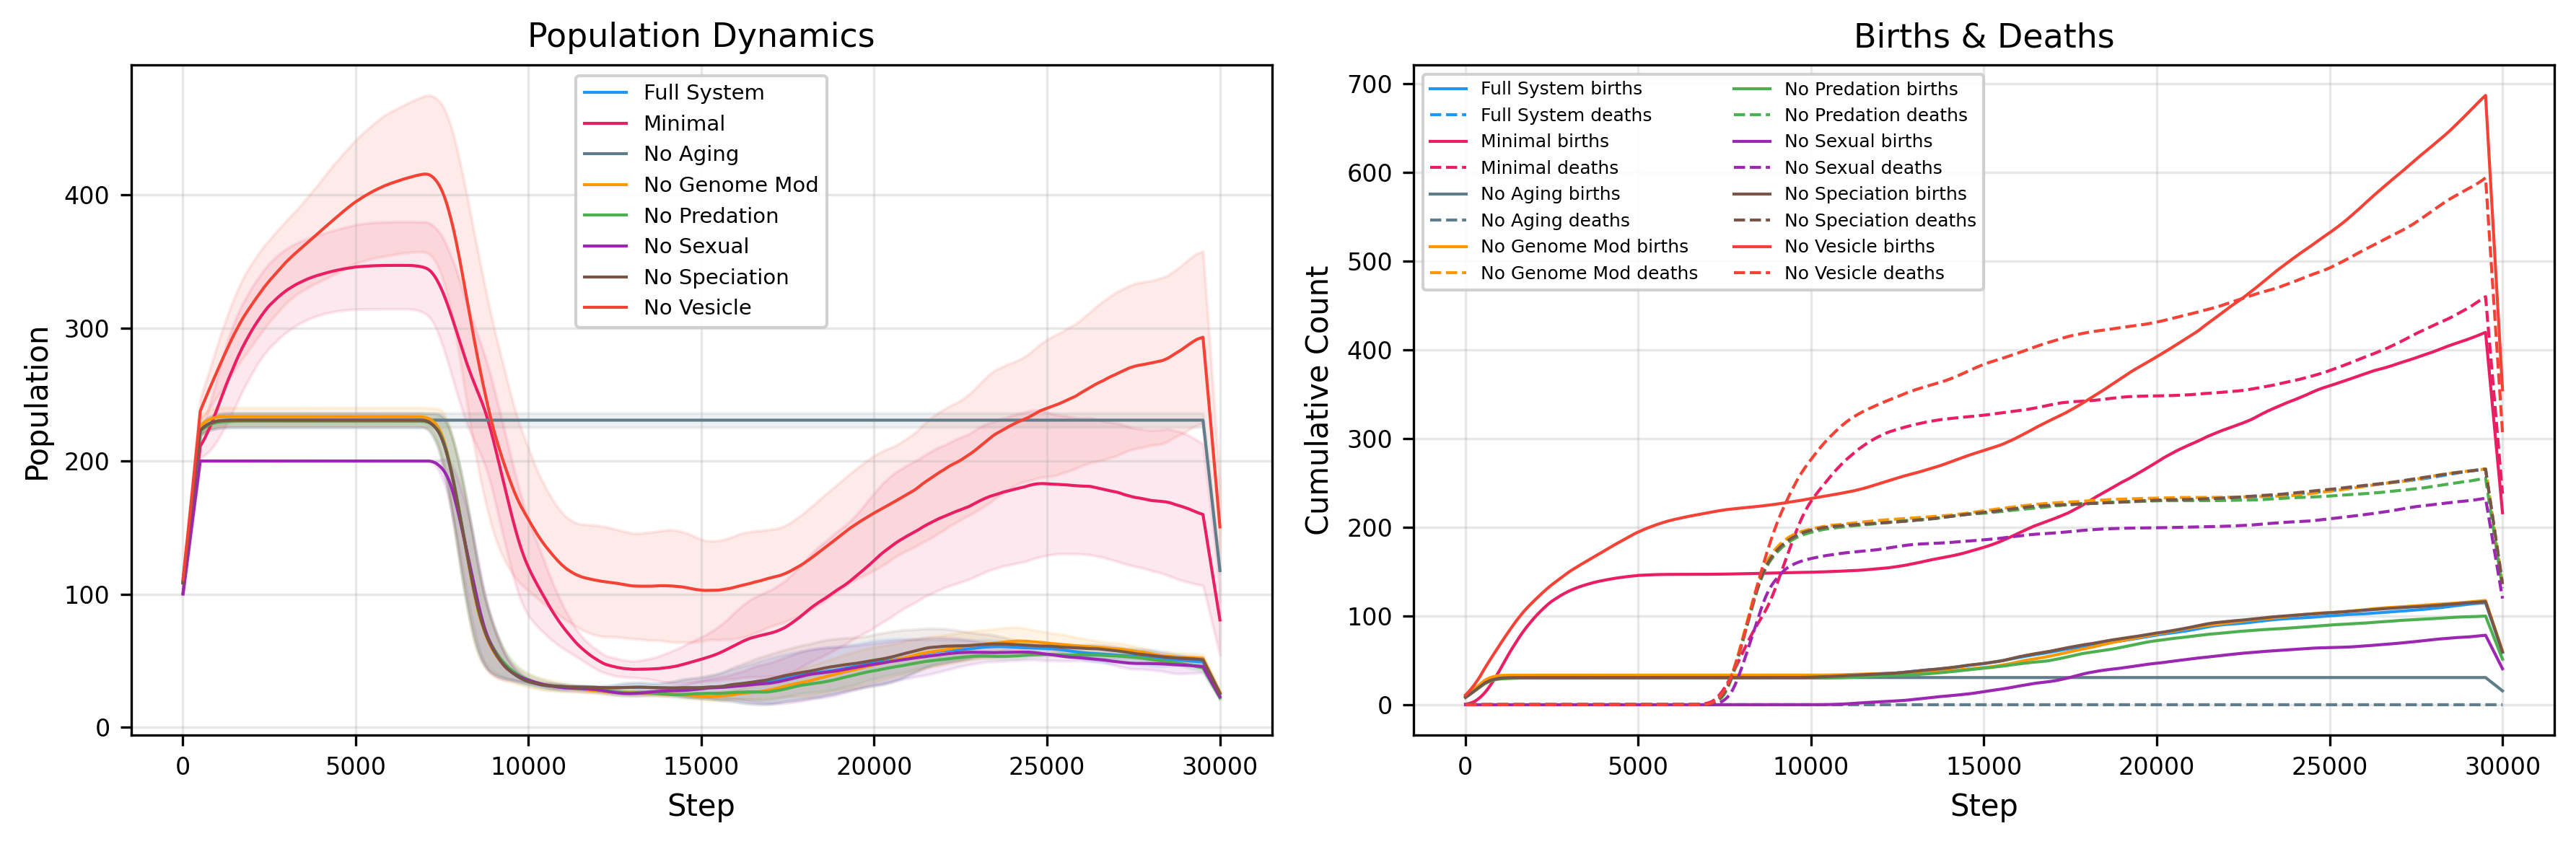
\includegraphics[width=\columnwidth]{results/figures/fig1_population.png}
  \caption{Population dynamics over 30{,}000 steps. The No Vesicle condition sustains $\sim$280 cells at steady state, while the Full System stabilizes near 51.}
  \label{fig:population}
\end{figure}

The most striking result is the dramatic effect of vesicle communication on population size (Figure~\ref{fig:population}).
The No Vesicle condition sustains approximately $280 \pm 10$ cells, whereas the Full System stabilizes at $51 \pm 2$---a five-fold reduction.
This is not a deficiency of the vesicle mechanism but rather an emergent consequence of the information-rich environment it creates.

Vesicle absorption modifies cell states (Eq.~\ref{eq:vesicle_absorb}), perturbing the phenotype vectors that determine nutrient affinity (Eq.~\ref{eq:nutrient}).
This state perturbation disrupts the alignment between cell phenotype and nutrient signature, effectively reducing feeding efficiency and creating a ``cost of communication.''
The system reaches a lower but more dynamic equilibrium in which cells must continuously adapt to a changing chemical landscape.

\subsection{Aging Is Essential for Generational Turnover}

\begin{figure}[t]
  \centering
  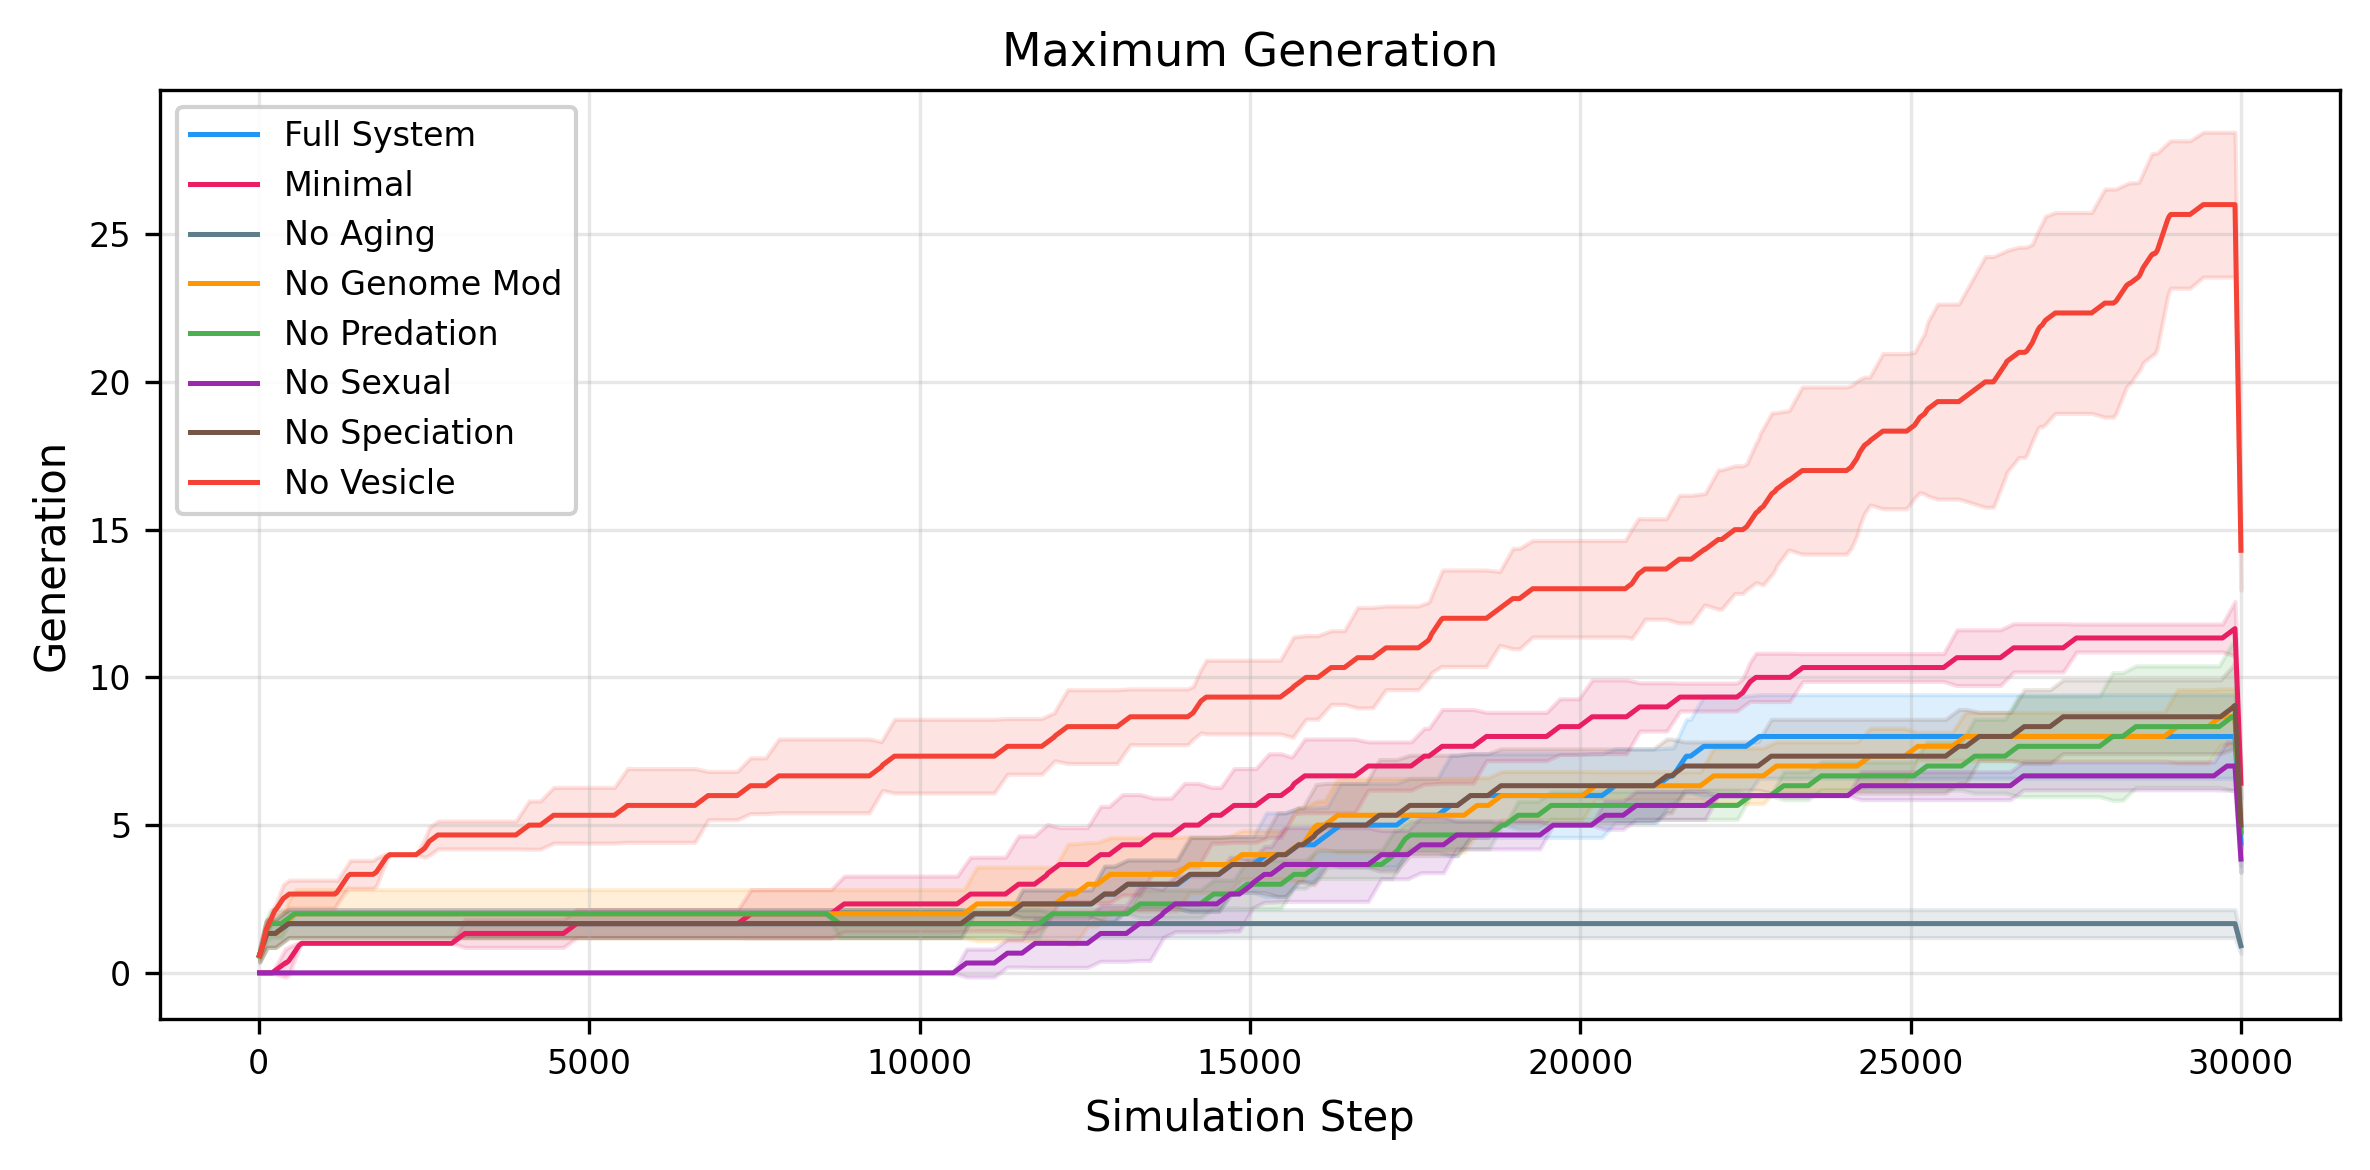
\includegraphics[width=\columnwidth]{results/figures/fig7_generations.png}
  \caption{Maximum generation reached over time. No Vesicle reaches generation 25; Full System reaches 8; No Aging is arrested at 2 with zero deaths.}
  \label{fig:generations}
\end{figure}

The No Aging condition is a dramatic outlier: the population stabilizes at $231 \pm 0$ cells with zero deaths across all seeds, and the maximum generation reaches only $1.7 \pm 0.5$ (Figure~\ref{fig:generations}).
Without aging pressure, the initial cohort of cells accumulates energy indefinitely, leaving no ecological room for offspring.
The 37, 24, and 31 births across three seeds (compared to 154, 90, and 107 for the Full System) confirm that reproduction is severely suppressed.
This result underscores that programmed senescence, even in its simplest form, is a prerequisite for evolutionary dynamics in energy-limited systems.

Among conditions with aging, the No Vesicle condition achieves the highest generational depth ($26.0 \pm 3.0$), consistent with its larger population providing more reproductive events.
The Full System reaches generation $8.0 \pm 1.7$, with fewer total births (117 $\pm$ 34 vs.\ 705 $\pm$ 216 for No Vesicle) but richer per-capita dynamics.

\subsection{Sexual Recombination Homogenizes Genomes}

\begin{figure}[t]
  \centering
  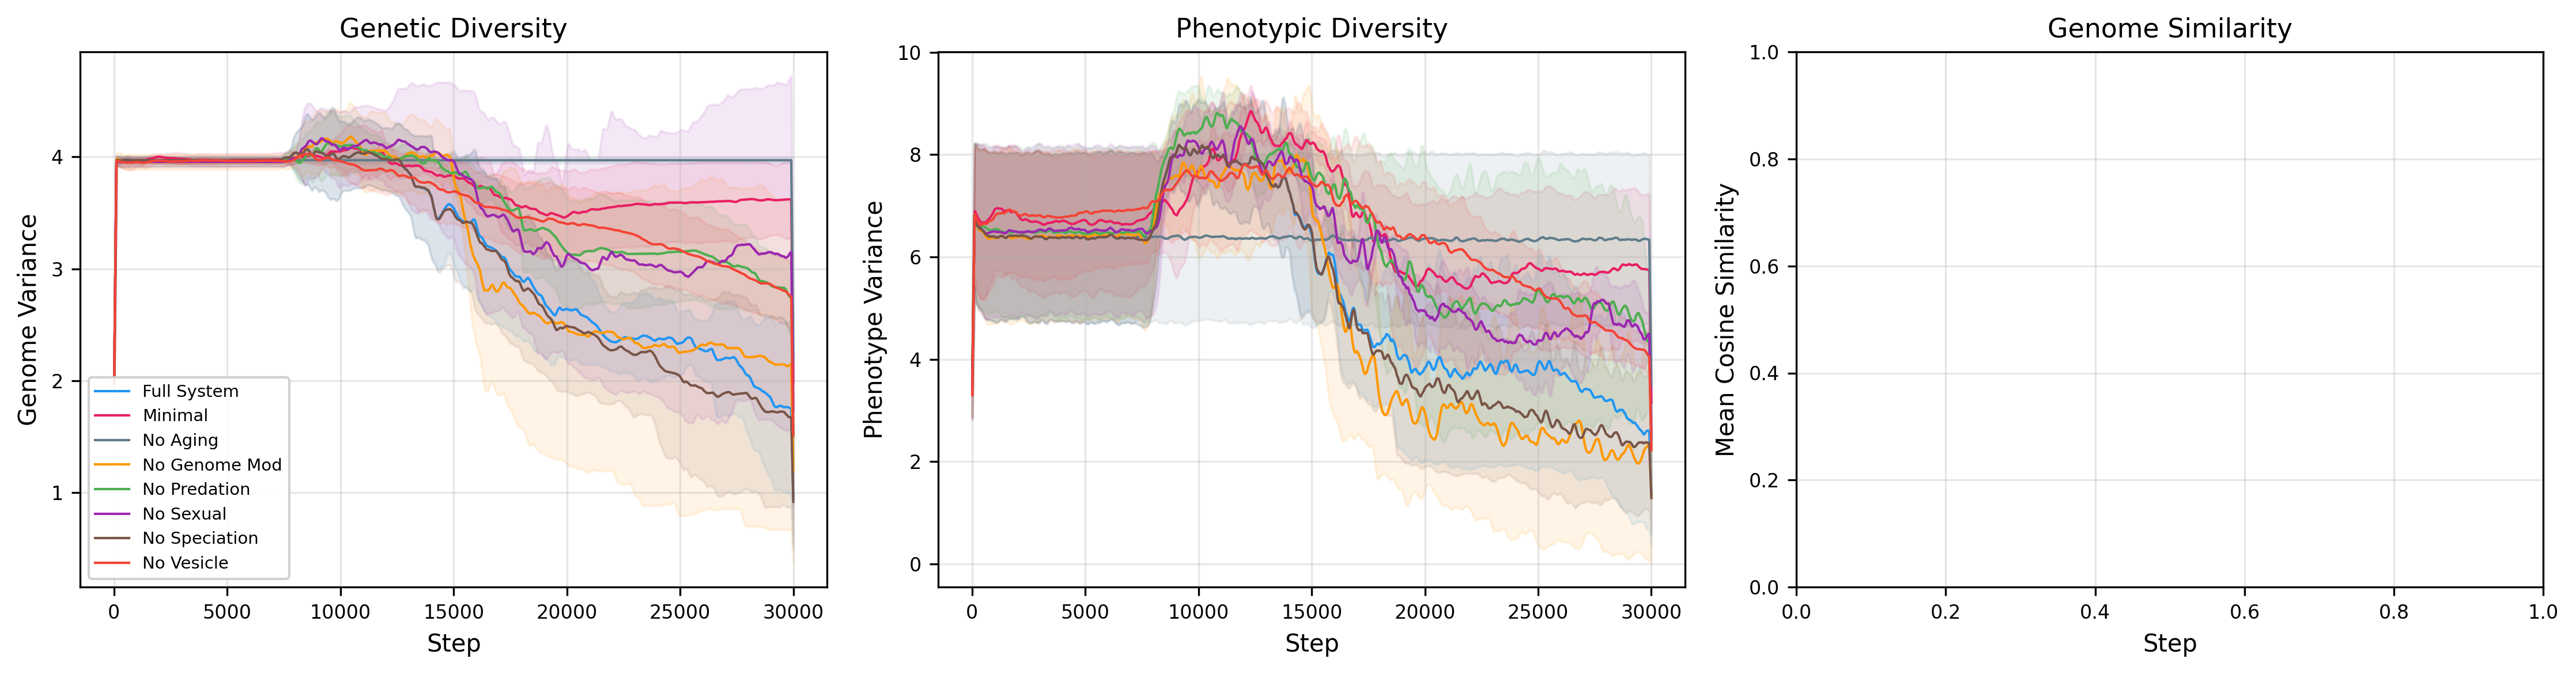
\includegraphics[width=\columnwidth]{results/figures/fig2_diversity.png}
  \caption{Genome and phenotype variance over time across ablation conditions.}
  \label{fig:diversity}
\end{figure}

Counterintuitively, removing sexual recombination \emph{increases} genome variance (No Sexual: $3.15 \pm 0.04$ vs.\ Full System: $1.95 \pm 0.16$).
The sexual recombination operator, constrained to parents with genome cosine similarity in $[0.3, 0.7]$, acts as a blending force that pulls genomes toward a shared centroid.
In the absence of sexual recombination, purely asexual division with mutation allows genomes to diverge along independent random walks, producing greater variance.

The phenotypic consequence is parallel: No Sexual shows the second-highest phenotype variance ($4.75 \pm 0.25$), behind only No Predation ($4.91 \pm 0.23$).
This suggests that the phenotypic diversity in the Full System is actively constrained by sexual recombination.

\subsection{Genome-Modulated Attention Shapes Phenotypic Variance}

\begin{figure}[t]
  \centering
  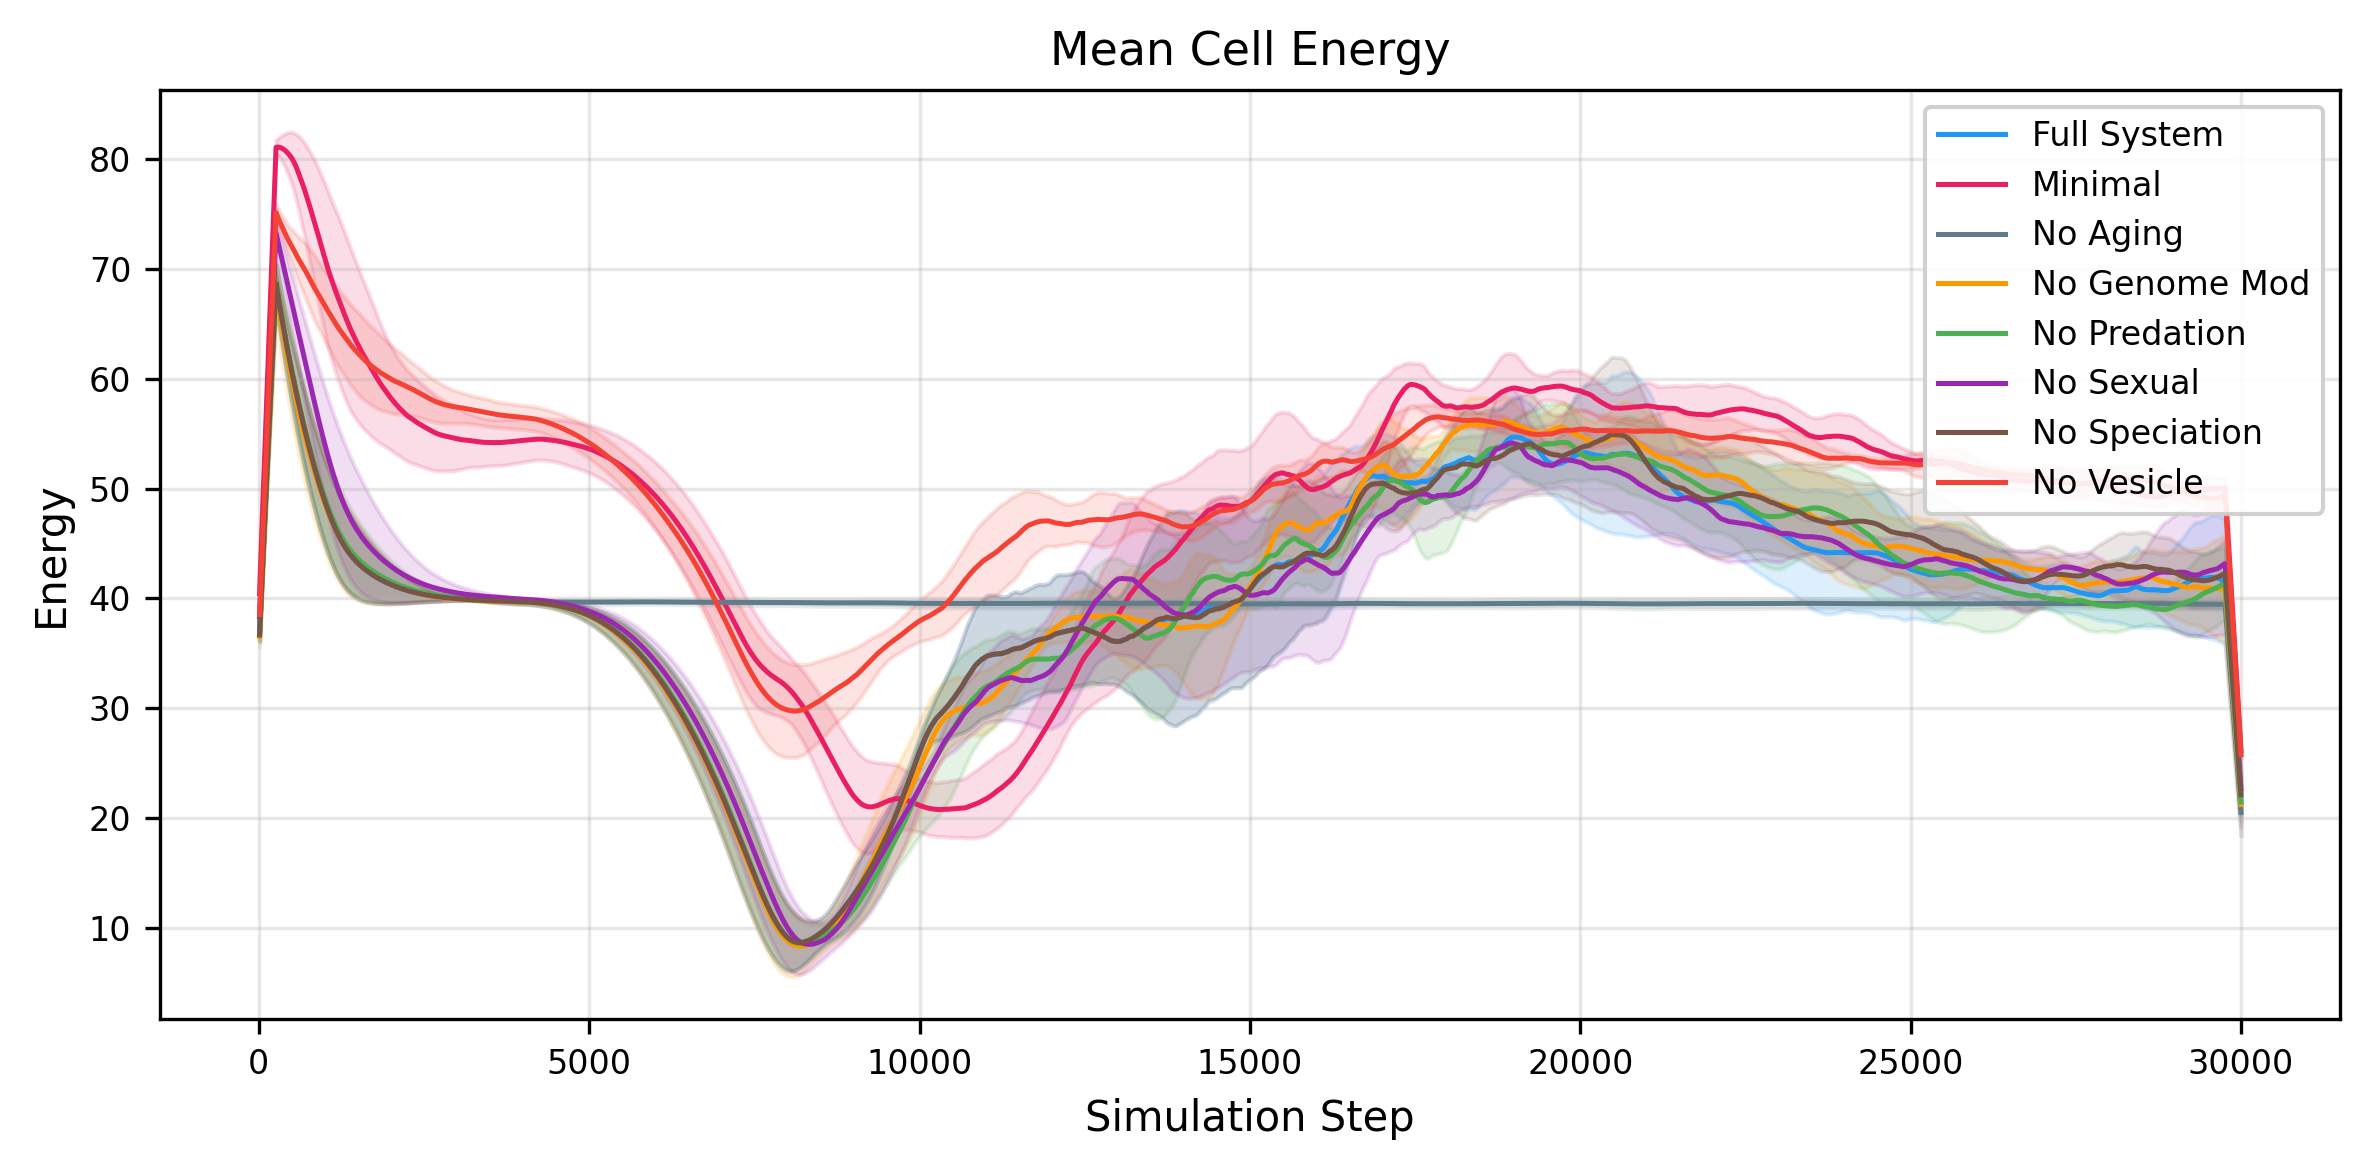
\includegraphics[width=\columnwidth]{results/figures/fig5_energy.png}
  \caption{Energy dynamics showing boom-bust cycles characteristic of the ecological interactions.}
  \label{fig:energy}
\end{figure}

Disabling genome modulation (fixing all $\alpha_q^{(h)} = \alpha_k^{(h)} = 0.5$) reduces phenotype variance from $3.00 \pm 0.29$ (Full System) to $2.19 \pm 0.14$---a 27\% decrease.
Population size is nearly unchanged ($54 \pm 3$ vs.\ $51 \pm 2$), indicating that genome modulation does not significantly affect survival but does meaningfully alter the behavioral repertoire.

This result confirms that the genome-modulated attention mechanism enables heritable phenotypic variation.
Different genome vectors produce different attention patterns, which in turn produce different movement, emission, and state-update behaviors, even though all cells share identical network weights.

\subsection{Speciation Pressure Reduces Genome Variance}

Disabling speciation pressure slightly decreases genome variance ($1.79 \pm 0.08$ vs.\ Full System $1.95 \pm 0.16$) and phenotype variance ($2.47 \pm 0.13$ vs.\ $3.00 \pm 0.29$).
The speciation pressure mechanism, which penalizes cells in genetically homogeneous neighborhoods, provides a modest diversifying force.
When removed, populations are free to converge without penalty, leading to reduced variance.

\subsection{Summary of Ablation Effects}

Figure~\ref{fig:energy} illustrates the energy dynamics across conditions, revealing the boom-bust cycles that characterize the ecological interactions in the system.
The Full System exhibits moderate cycling, while the No Aging condition shows monotonic energy accumulation.
The Minimal condition (no vesicles, no sexual recombination, no predation) maintains a population of $167 \pm 6$ with high diversity ($3.62 \pm 0.01$ genome variance), suggesting that the combination of vesicles and sexual recombination is responsible for the population compression observed in the Full System.

\begin{figure}[t]
  \centering
  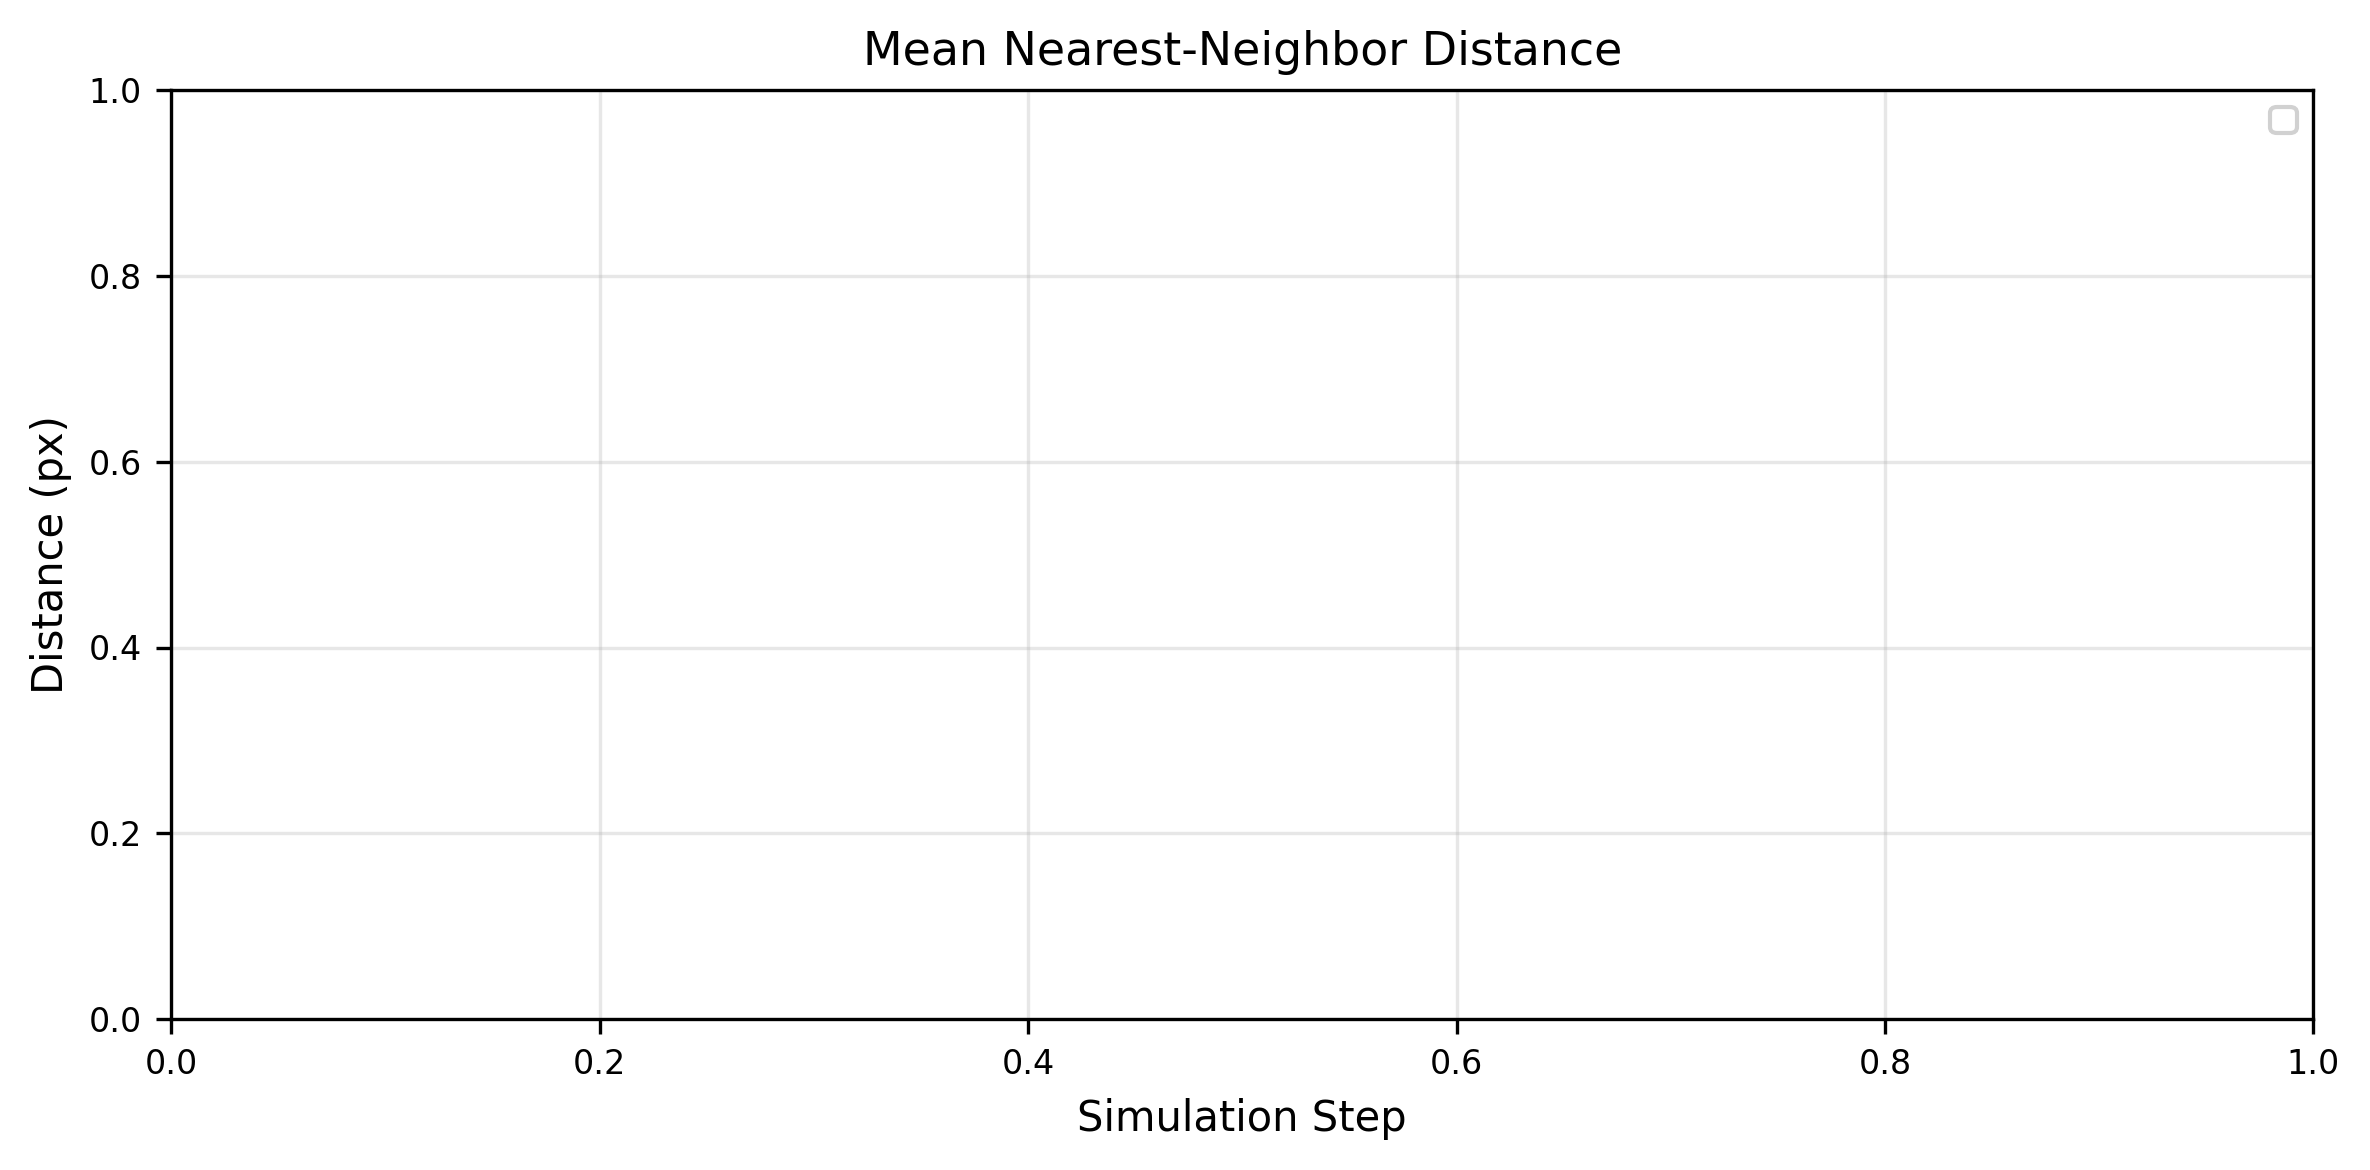
\includegraphics[width=\columnwidth]{results/figures/fig6_spatial.png}
  \caption{Spatial distribution of cells around nutrient sources, illustrating cluster formation.}
  \label{fig:spatial}
\end{figure}


% ============================================================================
\section{Discussion}
\label{sec:discussion}

\subsection{Vesicles as an Evolutionary Catalyst}

The central finding of this study is that vesicle communication, while reducing population size, creates a qualitatively different evolutionary regime.
In the No Vesicle condition, cells settle into stable nutrient niches and reproduce steadily, achieving high generational depth but relatively static behavioral patterns.
With vesicles, the environment becomes informationally richer: cells must contend not only with nutrient gradients and neighbors but also with an ambient field of diffusing neural states that continuously perturb their phenotypes.

This perturbation can be viewed as a form of \emph{environmental noise} that prevents the population from settling into fixed attractors.
While this reduces reproductive success in the short term, it may provide the variability necessary for long-term evolutionary innovation.
The analogy to biological extracellular vesicles (exosomes) is deliberate: in biological systems, vesicles carry proteins, lipids, and nucleic acids between cells, modulating recipient cell behavior in ways that are only beginning to be understood \cite{vanniel2018shedding,buddingh2017artificial}.
Recent work on synthetic compartments with life-like functionality \cite{buddingh2017artificial} further motivates the design of artificial vesicle communication as a bridge between biology and computation.

\subsection{The Paradox of Sexual Recombination}

The finding that sexual recombination reduces rather than increases genome diversity challenges conventional expectations from evolutionary biology.
In biological systems, sexual reproduction is understood to increase genetic diversity through recombination of parental chromosomes.
In our system, the constraining effect of the similarity window ($0.3 < \cos(\mathbf{g}_i, \mathbf{g}_j) < 0.7$) combined with the crossover operator acts as a centripetal force, averaging parental genomes and reducing the variance maintained by mutation alone.

This may be an artifact of the relatively small population sizes and short evolutionary timescales in our simulation.
In larger populations over longer runs, the interplay between sexual recombination, mutation, and selection might produce different outcomes.

\subsection{Limitations}

Several limitations of the current system should be acknowledged:

\begin{enumerate}
  \item \textbf{Random initial weights.} The Transformer brain's weights are randomly initialized and never updated.
  While this ensures that all behavioral variation comes from the genome and local context, it also means that the system cannot discover fundamentally new computational strategies.
  The brain operates as a fixed, randomly chosen function that is modulated by the genome but never improved.

  \item \textbf{No learning.} The absence of gradient-based or reward-based learning means that cells cannot adapt within their lifetimes.
  Combining evolution with lifetime learning (the Baldwin effect) could dramatically enrich the dynamics; population-based training \cite{jaderberg2017population} offers one promising approach for jointly optimizing hyperparameters and agent behavior across a population.

  \item \textbf{Short timescales.} At 30{,}000 steps and maximum generations of 8--29, the evolutionary dynamics are in an early, transient phase.
  Open-ended evolution, if achievable, would require substantially longer runs.

  \item \textbf{Small populations.} The steady-state populations of 50--280 cells are far below the scale at which complex ecological dynamics (food webs, trophic levels, competitive exclusion) typically emerge.
\end{enumerate}

\subsection{Visualization as Epistemic Tool and Aesthetic Object}

The visualization design serves a dual function that merits explicit discussion.
\emph{Epistemically}, the transparent-membrane rendering makes three otherwise invisible dynamics directly observable: (i) phenotypic clustering becomes spatial color segregation; (ii) vesicle communication appears as a visible ``chemical weather'' of glowing streaks overlaying the cell population; and (iii) the DNA barcode panel provides a phylogenetic snapshot at every frame, revealing speciation events as sudden barcode-pattern breaks within a nutrient cluster.
These channels collapse a high-dimensional dynamical system ($200+$ cells $\times$ 32-dim state $\times$ 16-dim genome) into a single frame that a human observer can parse in under a second.

\emph{Aesthetically}, the system exhibits visual qualities that arise without explicit design: the overlapping translucent membranes produce emergent interference patterns reminiscent of Ernst Haeckel's \emph{Kunstformen der Natur}; nutrient halos create depth-of-field layering; and the iridescent membrane shimmer evokes the optical properties of living cells under dark-field microscopy.
These are not cosmetic additions but \emph{natural consequences of mapping internal state to visual channels}---the beauty, such as it is, is a byproduct of information density.

This matters because ALife systems are increasingly exhibited as artworks \cite{sims1994evolving} and used as creative tools.
The capacity for real-time visual engagement is not peripheral to the scientific contribution: it determines whether researchers (and audiences) can develop the sustained attention necessary to notice rare, transient phenomena---an incipient species, a wave of vesicle-mediated coordination, a predation cascade---that would be invisible in log files alone.

\subsection{Future Work}

Several directions are promising for future development.
First, incorporating gradient-based meta-learning within individual cell lifetimes could enable Baldwinian evolution, where learned behaviors guide evolutionary search.
Second, scaling the system to thousands or millions of cells (potentially leveraging GPU acceleration via the existing CUDA/MPS support) would enable the emergence of richer ecological dynamics.
Third, extending the genome to modulate additional aspects of the brain architecture (e.g., feed-forward weights, layer normalization parameters) could increase the evolvability of the system.
Fourth, introducing an open-ended complexity measure \cite{lehman2011evolving} could help determine whether the system is capable of sustained evolutionary innovation---a central challenge in artificial life research \cite{packard2019overview,taylor2016open}.
Finally, the vesicle system could be extended toward a richer artificial chemistry \cite{banzhaf2015artificial} in which vesicle contents undergo compositional reactions, potentially enabling the emergence of self-replicating molecular patterns analogous to those studied by Hutton \cite{hutton2002evolvable}.


% ============================================================================
\section{Conclusion}
\label{sec:conclusion}

We have presented a novel artificial life system that combines Transformer-based neural controllers with genome-modulated attention and vesicle-mediated stigmergic communication.
Through a systematic ablation study across eight conditions, we have demonstrated that vesicle communication fundamentally reshapes population dynamics, reducing steady-state population size five-fold while creating richer energetic cycling; that aging pressure is essential for evolutionary progress; that sexual recombination, under the constraints of our similarity-gated crossover operator, homogenizes rather than diversifies genomes; and that genome-modulated attention produces measurable heritable variation in phenotypic behavior without requiring weight evolution.

These findings suggest that the combination of shared neural controllers, evolvable attention modulation, and diffusive chemical signaling provides a fertile substrate for exploring the emergence of complex adaptive behavior in artificial life systems.
The system bridges the gap between the rich individual-agent capabilities of modern deep learning architectures and the population-level evolutionary and ecological dynamics that have traditionally been the province of simpler agent models.


% ============================================================================
\section*{Acknowledgments}

This work was supported by the Digital Nature Group at the University of Tsukuba. The simulation was implemented in Python using PyTorch and Pygame.

\bibliographystyle{plainnat}
\bibliography{refs}

\end{document}
